%%%%%%%%%%%%%%%%%%%%% chapter.tex %%%%%%%%%%%%%%%%%%%%%%%%%%%%%%%%%
%
% sample chapter
%
% Use this file as a template for your own input.
%
%%%%%%%%%%%%%%%%%%%%%%%% Springer-Verlag %%%%%%%%%%%%%%%%%%%%%%%%%%
%\motto{Use the template \emph{chapter.tex} to style the various elements of your chapter content.}
\chapter{Example D: two sector economy with durable and non-durable demand}
\chaptermark{Durable and non-durable}
\label{chap:two_sector_durable} % Always give a unique label
% use \chaptermark{}
% to alter or adjust the chapter heading in the running head

\abstract*{[NEED TO ADD ABSTRACT HERE]}

%% \abstract{Each chapter should be preceded by an abstract (10--15 lines long) that summarizes the content. The abstract will appear \textit{online} at \url{www.SpringerLink.com} and be available with unrestricted access. This allows unregistered users to read the abstract as a teaser for the complete chapter. As a general rule the abstracts will not appear in the printed version of your book unless it is the style of your particular book or that of the series to which your book belongs.\newline\indent
%% Please use the 'starred' version of the new Springer \texttt{abstract} command for typesetting the text of the online abstracts (cf. source file of this chapter template \texttt{abstract}) and include them with the source files of your manuscript. Use the plain \texttt{abstract} command if the abstract is also to appear in the printed version of the book.}

%% Use the template \emph{chapter.tex} together with the Springer document class SVMono (monograph-type books) or SVMult (edited books) to style the various elements of your chapter content in the Springer layout.


[INSERT QUOTE FROM G-R]

We now extend the two-sector economy from Example C by distinguishing between flows from sector $i$ into sector $j$ which are being processed---such as the tailor's cloth and thread, to use Georgescu-Roegen's example---and are destined to leave in the products of that sector, $\dot{T}_{j}$ (except for some proportion of wastage) and flows which are doing the processing---the tailor's needle and labor. The processed flows we term \emph{resource} flows, $\dot{R}_{ij}$ and may comprise either direct energy or energy embodied in goods or services. We assume that these do not accumulate within a sector, such that $\frac{\textrm{d}R}{\textrm{dt}} = 0$.

\begin{figure}[h!]
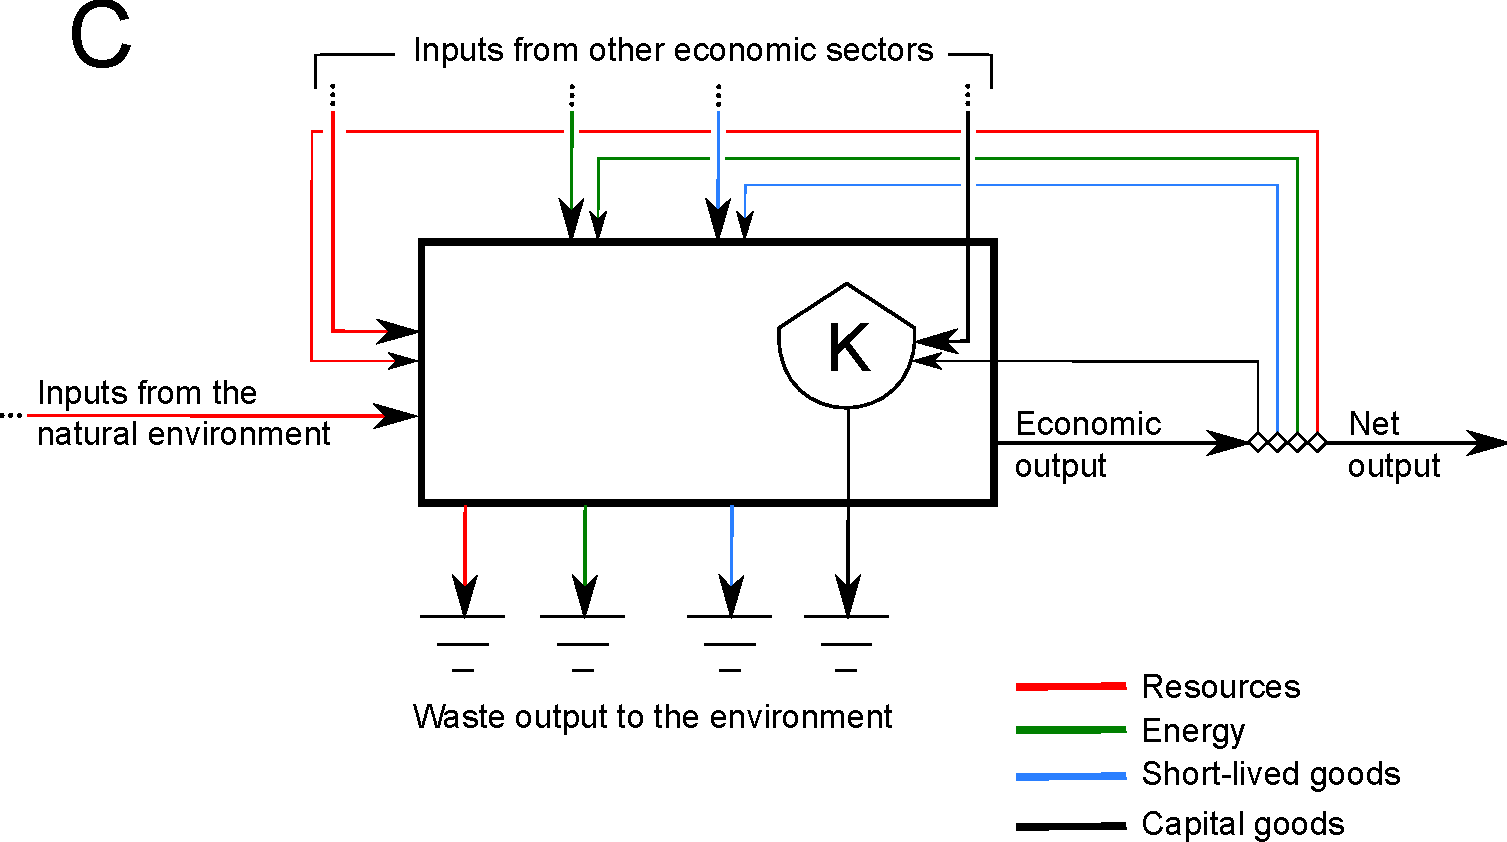
\includegraphics[width=1.0\linewidth]{Chapter_Example_D/images/Basic_unit_C.pdf}
\caption{Flows of resources (red arrows), direct energy ($\dot{E}$, green arrows), short-lived goods (blue arrows), capital goods (black arrows) and waste flows including waste heat ($\dot{Q}$) for a single economic sector. Flows of capital $\dot{K}$ are able to accumulate within the sector; no other flows may accumulate.}
\label{fig:basic_unit_C}
\end{figure}

We also introduce a distinction between two types of embodied energy flows: short-lived, non-durable goods (S), such as packaging, newspapers or the embodied energy content of direct energy flows and long-lived, durable goods (L), such as appliances, capital equipment, roads or buildings. In reality, (as the names suggest) the distinction between short- and long-lived goods is really one of degree rather than a difference in kind such that the distribution in lifetime of goods stretches from a matter of hours or days for some intermediate goods right up to thousands of years for some structures still in use today \cite{Leask2012}. We assume that there is no accumulation of short-lived goods within the economy or society, such that $\frac{\textrm{d}S}{\textrm{dt}} = 0$.  

These flows are shown in Figure XXXX for our two sector economy. Resource flows enter into the sector from the left and products leave from the right, processing flows enter from the top and waste flows leave from the bottom. We may now define the following relationships:

\begin{figure}[h!]
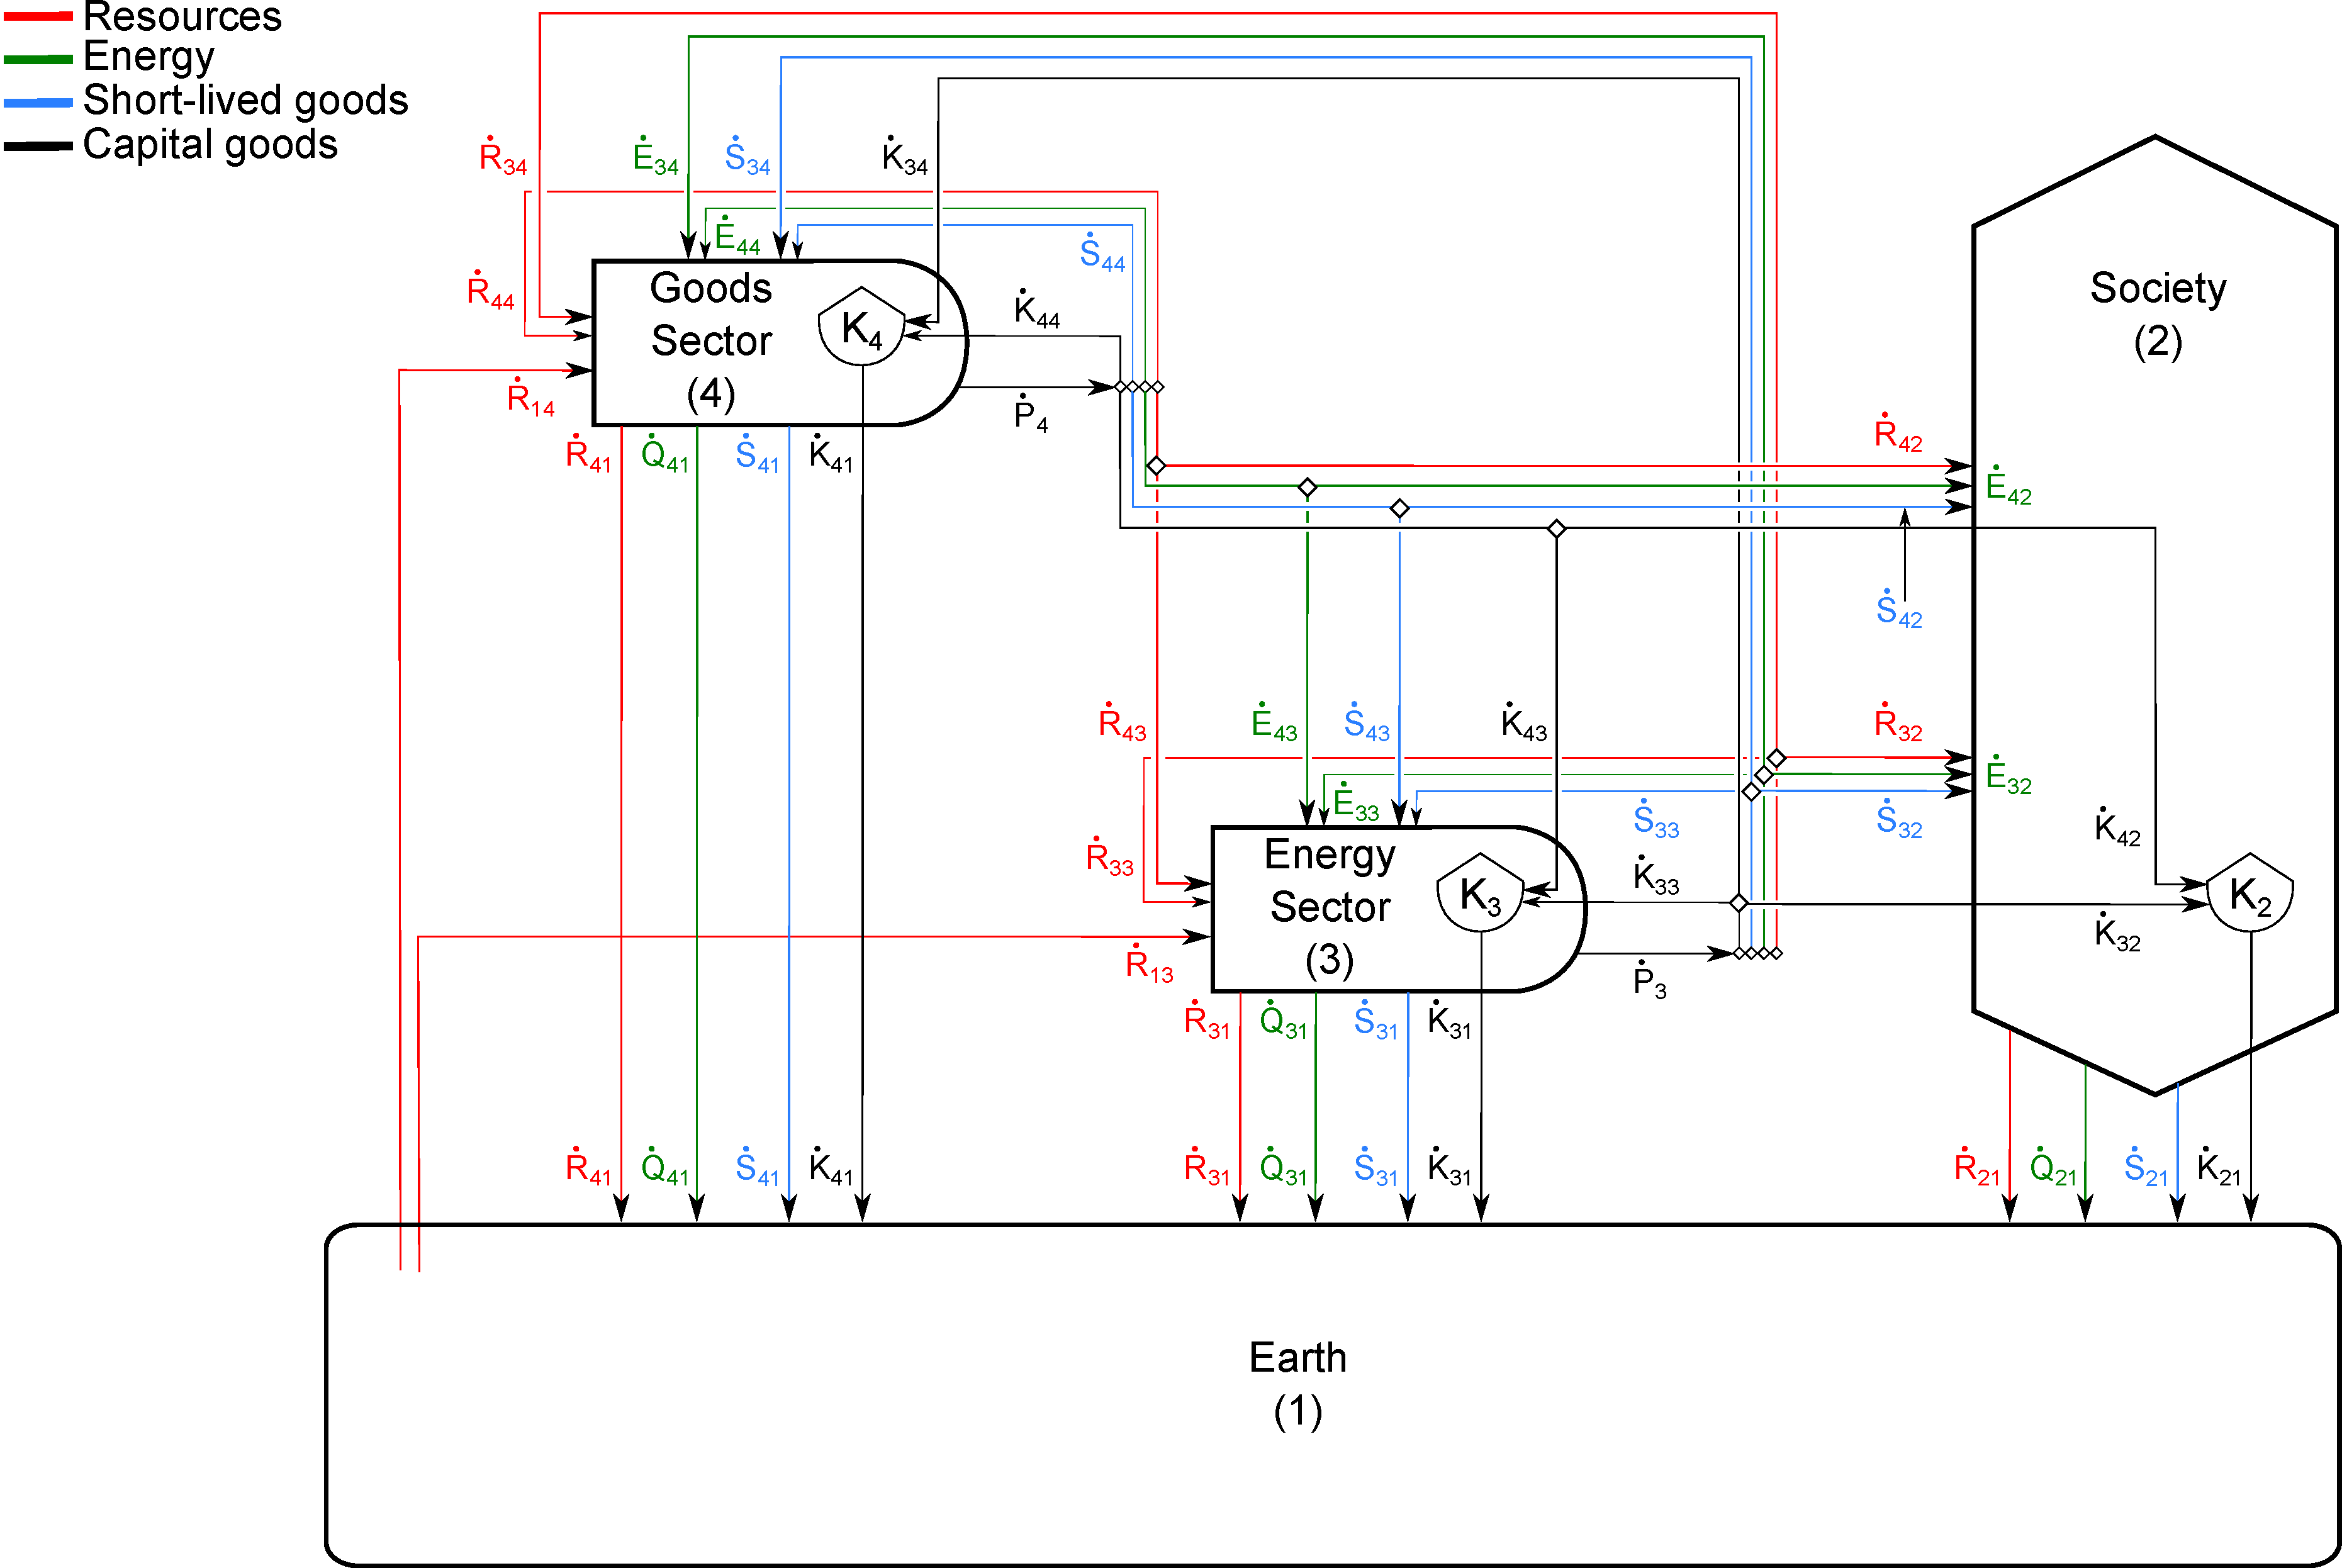
\includegraphics[width=1.0\linewidth]{Chapter_Example_D/images/PERKS_two_sector.pdf}
\caption{Flows of resources (red arrows), direct energy ($\dot{E}$, green arrows), short-lived goods (blue arrows), capital goods (black arrows) and waste flows including waste heat ($\dot{Q}$) for a two sector economy. Flows of capital $\dot{K}$ are able to accumulate within the sector; no other flows may accumulate.}
\label{fig:PERKS}
\end{figure}

\begin{equation}\label{eq:D_def_S_L}
B_{j} \equiv S_{j} + L_{j} = L_{j}
\end{equation}

%\begin{equation}\label{eq:D_def_dot_S_L}
%\dot{B} = \dot{S} + \dot{L} = \zeta\dot{B} + (1-\zeta)\dot{B}
%\end{equation}


\begin{equation}\label{eq:D_def_acc_S_L}
\frac{\textrm{d}B_{j}}{\textrm{dt}} =\frac{\textrm{d}S_{j}}{\textrm{dt}} + \frac{\textrm{d}L_{j}}{\textrm{dt}} = \frac{\textrm{d}L_{j}}{\textrm{dt}}
\end{equation}

We assume that all non-resource, energy flows $\dot{E}_{ij}$ are degraded to waste heat $\dot{Q}_{j1}$ by the processes of the sector, such that:

\begin{equation}\label{eq:D_E_balance}
\sum_{i} \dot{E}_{ij} = \dot{Q}_{j1}
\end{equation}

Similarly, we assume that all short-lived embodied energy flows $\dot{S}_{ij}$ are degraded to waste $\dot{S}_{j1}$ by the processes of the sector, such that:

\begin{equation}\label{eq:D_S_balance}
\sum_{i} \dot{S}_{ij} = \dot{S}_{j1}
\end{equation}

Since long-lived embodied energy flows, $\dot{L}_{ij}$ may accumulate with a sector, we can define that:

\begin{equation}\label{eq:D_L_balance}
\sum_{i} \dot{L}_{ij} = \dot{L}_{j1} + \frac{\textrm{d}L_{j}}{\textrm{dt}}
\end{equation}

%Given equations \ref{eq:D_E_balance} - \ref{eq:D_L_balance}, we may now stipulate that any resource flows into a sector, $\dot{R}_{ij}$, must either leave as waste flows to the earth $\dot{R}_{j1}$, or as part of the product from that sector $\dot{T}_{j}$, such that:
%
%\begin{equation}\label{eq:D_T_balance}
%\sum_{i} \dot{R}_{ij} = \dot{R}_{j1} + \dot{T}_{j}
%\end{equation}

%%%%%%%%%% Example D %%%%%%%%%%
\section{First Law of Thermodynamics}
%%%%%%%%%%

As before, the First Law of Thermodynamics requires that energy is conserved around each sector of the economy as well as around the Earth (1) and Society (2) as shown in Figure \ref{}. 

The First Law of Thermodynamics around the Earth (1), Society (2), the Energy sector (3) and Goods and Services sector (4) gives

\begin{equation} \label{eq:D-CV_E_dot_1}
	\frac{\mathrm{d}E_{1}}{\mathrm{d}t} 	 =  \dot{Q}_{21} + \dot{Q}_{31} + \dot{Q}_{41} - \dot{E}_{13} - \dot{E}_{14},
\end{equation}

\begin{equation} \label{eq:D-CV_E_dot_2}
	\frac{\mathrm{d}E_{2}}{\mathrm{d}t} 	 = \dot{E}_{32}  + \dot{E}_{42} - \dot{Q}_{21},
\end{equation}

\begin{equation} \label{eq:D-CV_E_dot_3}
	\frac{\mathrm{d}E_{3}}{\mathrm{d}t} 	 = \dot{E}_{13} + \dot{E}_{33} + \dot{E}_{43} - \dot{E}_{3} - \dot{Q}_{31}.
\end{equation}

\noindent and 

\begin{equation} \label{eq:D-CV_E_dot_4}
	\frac{\mathrm{d}E_{4}}{\mathrm{d}t} 	 = \dot{E}_{14} + \dot{E}_{34} + \dot{E}_{44} - \dot{E}_{4} - \dot{Q}_{41}.
\end{equation}

As in Examples A and B, we can set the accumulation of direct energy to zero.

\begin{equation} \label{eq:D-CV_E_dot_1_SS}
	0 =  \dot{Q}_{21} + \dot{Q}_{31} + \dot{Q}_{41} - \dot{E}_{13} - \dot{E}_{14}
\end{equation}

\begin{equation} \label{eq:D-CV_E_dot_2_SS}
	0  = \dot{E}_{32}  + \dot{E}_{42} - \dot{Q}_{21}
\end{equation}

\begin{equation} \label{eq:D-CV_E_dot_3_SS}
	0 = \dot{E}_{13} + \dot{E}_{33} + \dot{E}_{43} - \dot{E}_{3} - \dot{Q}_{31}
\end{equation}

\noindent and 

\begin{equation} \label{eq:D-CV_E_dot_4_SS}
	0 = \dot{E}_{14} + \dot{E}_{34} + \dot{E}_{44} - \dot{E}_4 - \dot{Q}_{41}
\end{equation}


%%%%%%%%%% Example D %%%%%%%%%%
\section{Total energy accounting}
%%%%%%%%%%

Accounting for accumulation of total energy and using the assumption that total energy is conserved, we can write the following equations.

\begin{equation} \label{eq:D-CV_T_1}
	\frac{\mathrm{d}T_{1}}{\mathrm{d}t} 	 = \dot{T}_{21} + \dot{T}_{31} + \dot{T}_{41} - \dot{T}_{13} - \dot{T}_{14},
\end{equation}

\begin{equation} \label{eq:D-CV_T_2}
	\frac{\mathrm{d}T_{2}}{\mathrm{d}t} 	 = \dot{T}_{32} + \dot{T}_{42} - \dot{T}_{21},
\end{equation}

\begin{equation} \label{eq:D-CV_T_3}
	\frac{\mathrm{d}T_{3}}{\mathrm{d}t} 	 = \dot{T}_{13} + \dot{T}_{33} + \dot{T}_{43} - \dot{T}_{3} - \dot{T}_{31},
\end{equation}

\noindent and 

\begin{equation} \label{eq:D-CV_T_4}
	\frac{\mathrm{d}T_{4}}{\mathrm{d}t} 	 = \dot{T}_{14} + \dot{T}_{34} + \dot{T}_{44} - \dot{T}_{4} - \dot{T}_{41}.
\end{equation}


%%%%%%%%%% Example D %%%%%%%%%%
\section{Embodied energy accounting}
%%%%%%%%%%

Given that $\frac{\mathrm{d}E_{i}}{\mathrm{d}t} = \frac{\mathrm{d}R_{i}}{\mathrm{d}t} = \frac{\mathrm{d}S_{i}}{\mathrm{d}t} = 0$, we note that $\frac{\mathrm{d}T_i}{\mathrm{d}t} = \frac{\mathrm{d}L_i}{\mathrm{d}t}$. Substituting $\dot{T} = \dot{R} + \dot{E} + \dot{S} + \dot{L}$ into the total energy accounting equations gives

\begin{equation} \label{eq:D-CV_dB_1}
	\frac{\mathrm{d}L_{1}}{\mathrm{d}t} 	 = \dot{E}_{21} + \dot{S}_{21} + \dot{L}_{21} + \dot{R}_{31} + \dot{E}_{31} + \dot{S}_{31} + \dot{L}_{31} + \dot{R}_{41} + \dot{E}_{41} + \dot{S}_{41} + \dot{L}_{41} - \dot{R}_{13} - \dot{R}_{14},
\end{equation}

\begin{equation} \label{eq:D-CV_dB_2}
	\frac{\mathrm{d}L_{2}}{\mathrm{d}t} 	 = \dot{E}_{32} + \dot{S}_{32} + \dot{L}_{32} + \dot{E}_{42} + \dot{S}_{42} + \dot{L}_{42} - \dot{E}_{21} - \dot{S}_{21} - \dot{L}_{21},
\end{equation}

\begin{equation} \label{eq:D-CV_dB_3}
	\frac{\mathrm{d}L_{3}}{\mathrm{d}t} 	 = \dot{R}_{13} + \dot{R}_{33} + \dot{E}_{33} + \dot{S}_{33} + \dot{L}_{33} + \dot{R}_{43} + \dot{E}_{43} + \dot{S}_{43} + \dot{L}_{43} - \dot{T}_{3} - \dot{R}_{31} - \dot{E}_{31} - \dot{S}_{31} - \dot{L}_{31},
\end{equation}

\noindent and 

\begin{equation} \label{eq:D-CV_dB_4}
	\frac{\mathrm{d}L_{4}}{\mathrm{d}t} 	 = \dot{R}_{14} + \dot{R}_{34} + \dot{E}_{34} + \dot{S}_{34} + \dot{L}_{34} + \dot{R}_{44} + \dot{E}_{44} + \dot{S}_{44} + \dot{L}_{44} - \dot{T}_{4} - \dot{R}_{41} - \dot{E}_{41} - \dot{S}_{41} - \dot{L}_{41}.
\end{equation}

Substituting the First Law of Thermodynamics (Equations \ref{eq:D-CV_E_dot_1_SS} through \ref{eq:D-CV_E_dot_4_SS}) into the total energy accounting equations (Equations \ref{eq:D-CV_dB_1} through \ref{eq:D-CV_dB_4}) gives embodied energy accounting equations for Example D.

\begin{equation} \label{eq:D-embodied_acct_1}
	\frac{\mathrm{d}L_{1}}{\mathrm{d}t} 	 = \dot{S}_{21} + \dot{L}_{21} + \dot{R}_{31} + \dot{S}_{31} + \dot{L}_{31} + \dot{R}_{41} +\dot{S}_{41} + \dot{L}_{41} - \dot{Q}_{21} - \dot{Q}_{31} - \dot{Q}_{41}
\end{equation}

\begin{equation} \label{eq:D-embodied_acct_2}
	\frac{\mathrm{d}L_{2}}{\mathrm{d}t} 	 = \dot{S}_{32} + \dot{L}_{32} + \dot{S}_{42} + \dot{L}_{42} + \dot{Q}_{21} - \dot{S}_{21} - \dot{L}_{21}
\end{equation}

\begin{equation} \label{eq:D-embodied_acct_3}
	\frac{\mathrm{d}L_{3}}{\mathrm{d}t} 	 = \dot{S}_{33} + \dot{L_33} + \dot{S}_{43} + \dot{L}_{43} + \dot{Q}_{31} + \dot{E}_{3} - \dot{T}_{3} - \dot{R}_{31} - \dot{S}_{31} - \dot{L}_{31}
\end{equation}

\begin{equation} \label{eq:D-embodied_acct_4}
	\frac{\mathrm{d}L_{4}}{\mathrm{d}t} 	 = \dot{S}_{34} + \dot{L_34} + \dot{S}_{44} + \dot{L}_{44} + \dot{Q}_{41} + \dot{E}_{4} - \dot{T}_{4} - \dot{R}_{41} - \dot{S}_{41} - \dot{L}_{41}
\end{equation}

[MIK ENDED HERE - MAR 27, 2013]

%Again remembering that $\frac{\textrm{d}E_{i}}{\textrm{dt}} = \dot{E}_{i1} = 0$ we can substitute \ref{eq:D_first_law} into \ref{eq:D_total_energy} to obtain:
%
%\begin{equation}\label{eq:D_emb_energy}
%\frac{\textrm{d}B_{i}}{\textrm{dt}} = \sum_{j}\dot{B}{ji} - \dot{B}_{i} - \dot{B}_{i1} + \dot{Q}_{i1}
%\end{equation}
%
%Remembering that $\frac{\textrm{d}S_{i}}{\textrm{dt}} = 0$ and $\frac{\textrm{d}B_{i}}{\textrm{dt}} = \frac{\textrm{d}S_{i}}{\textrm{dt}} + \frac{\textrm{d}L_{i}}{\textrm{dt}} = \frac{\textrm{d}L_{i}}{\textrm{dt}}$, we may simplify equation \ref{eq:D_emb_energy} to:
%
%\begin{equation}\label{eq:D_emb_energy_dL}
%\frac{\textrm{d}L_{i}}{\textrm{dt}} = \sum_{j}\dot{B}{ji} - \dot{B}_{i} - \dot{B}_{i1} + \dot{Q}_{i1}
%\end{equation}

%Given that $\frac{\mathrm{d}E_{i}}{\mathrm{d}t} = \frac{\mathrm{d}S_{i}}{\mathrm{d}t} = 0$, we again note that $\frac{\mathrm{d}T_i}{\mathrm{d}t} = \frac{\mathrm{d}B_i}{\mathrm{d}t} = \frac{\mathrm{d}L_{i}}{\mathrm{d}t}$. Substituting $\dot{T} = \dot{E} + \dot{B} = \dot{E} + \dot{S} + \dot{L}$ into the total energy accounting equations gives
%
%\begin{equation} \label{eq:D-CV_dB_1}
%	\frac{\mathrm{d}L_{1}}{\mathrm{d}t} 	 = \dot{E}_{21} + \dot{S}_{21} + \dot{L}_{21}+ \dot{E}_{31} + \dot{S}_{31} + \dot{L}_{31} + \dot{E}_{41} + \dot{S}_{41} + \dot{L}_{41} - \dot{E}_{13} - \dot{S}_{13} - \dot{L}_{13} - \dot{E}_{14} - \dot{S}_{14} - \dot{L}_{14},
%\end{equation}
%
%\begin{equation} \label{eq:D-CV_dB_2}
%	\frac{\mathrm{d}L_{2}}{\mathrm{d}t} 	 = \dot{E}_{32} + \dot{S}_{32} + \dot{L}_{32} + \dot{E}_{42} + \dot{S}_{42} + \dot{L}_{42} - \dot{E}_{21} - \dot{S}_{21} - \dot{L}_{21},
%\end{equation}
%
%\begin{equation} \label{eq:D-CV_dB_3}
%	\frac{\mathrm{d}L_{3}}{\mathrm{d}t} 	 = \dot{E}_{13} + \dot{S}_{13} + \dot{L}_{13} + \dot{E}_{33} + \dot{S}_{33} + \dot{L}_{33}+ \dot{E}_{43} + \dot{S}_{43} + \dot{L}_{43} - \dot{E}_{3} - \dot{S}_{3} - \dot{L}_{3} - \dot{E}_{31} - \dot{S}_{31} - \dot{L}_{31},
%\end{equation}
%
%\noindent and 
%
%\begin{equation} \label{eq:D-CV_dB_4}
%	\frac{\mathrm{d}L_{4}}{\mathrm{d}t} 	 = \dot{E}_{14} + \dot{S}_{14} + \dot{L}_{14} + \dot{E}_{34} + \dot{S}_{34} + \dot{L}_{34}+ \dot{E}_{44} + \dot{S}_{44} + \dot{L}_{44} - \dot{E}_{4} - \dot{S}_{4} - \dot{L}_{4} - \dot{E}_{41} - \dot{S}_{41} - \dot{L}_{41}.
%\end{equation}
%
%Substituting the First Law of Thermodynamics (Equations \ref{eq:C-CV_E_dot_1_SS} through \ref{eq:C-CV_E_dot_4_SS}) into the total energy accounting equations (Equations \ref{eq:D-CV_dB_1} through \ref{eq:D-CV_dB_4}) gives embodied energy accounting equations for Example D.
%
%\begin{equation} \label{eq:D-embodied_acct_1}
%	\frac{\mathrm{d}L_{1}}{\mathrm{d}t} 	 = \dot{S}_{21} + \dot{L}_{21} + \dot{S}_{31} + \dot{L}_{31} + \dot{S}_{41} + \dot{L}_{41} - \dot{S}_{13} - \dot{L}_{13} - \dot{S}_{14} -  \dot{L}_{14} - \dot{Q}_{21} - \dot{Q}_{31} - \dot{Q}_{41}
%\end{equation}
%
%\begin{equation} \label{eq:D-embodied_acct_2}
%	\frac{\mathrm{d}L_{2}}{\mathrm{d}t} 	 = \dot{S}_{32} +  \dot{L}_{32} + \dot{S}_{42} +  \dot{L}_{42} + \dot{Q}_{21} - \dot{S}_{21} -  \dot{L}_{21}
%\end{equation}
%
%\begin{equation} \label{eq:D-embodied_acct_3}
%	\frac{\mathrm{d}L_{3}}{\mathrm{d}t} 	 = \dot{S}_{13} +  \dot{L}_{13} + \dot{S}_{33} +  \dot{L}_{33} + \dot{S}_{43} +  \dot{L}_{43} + \dot{Q}_{31} - \dot{S}_{3} -  \dot{L}_{3} - \dot{S}_{31} -  \dot{L}_{31}
%\end{equation}
%
%\begin{equation} \label{eq:D-embodied_acct_4}
%	\frac{\mathrm{d}L_{4}}{\mathrm{d}t}	 = \dot{S}_{14} +  \dot{L}_{14} + \dot{S}_{34} +  \dot{L}_{34} + \dot{S}_{44} +  \dot{L}_{44} + \dot{Q}_{41} - \dot{S}_{4} -  \dot{L}_{4} - \dot{S}_{41} -  \dot{L}_{41}
%\end{equation}
%
%To verify the above derivation, we sum Equations \ref{eq:D-embodied_acct_1} through \ref{eq:D-embodied_acct_4} and use the following identities:
%
%\begin{equation} \label{eq:D-S_sum_3_output}
%	\dot{S}_3 = \dot{S}_{32} + \dot{S}_{33} + \dot{S}_{34}
%\end{equation}
%
%\begin{equation} \label{eq:D-L_sum_3_output}
%	\dot{L}_3 = \dot{L}_{32} + \dot{L}_{33} + \dot{L}_{34}
%\end{equation}
%
%\begin{equation} \label{eq:D-S_sum_4_output}
%	\dot{S}_4 = \dot{S}_{42} + \dot{S}_{43} + \dot{S}_{44};
%\end{equation}
%
%\noindent and
%
%\begin{equation} \label{eq:D-L_sum_4_output}
%	\dot{L}_4 = \dot{L}_{42} + \dot{L}_{43} + \dot{L}_{44};
%\end{equation}
%
%\noindent to obtain
%
%\begin{equation} \label{eq:D-B_sums_to_zero}
%	\frac{\mathrm{d}B_{1}}{\mathrm{d}t} + \frac{\mathrm{d}B_{2}}{\mathrm{d}t} + \frac{\mathrm{d}B_{3}}{\mathrm{d}t} + \frac{\mathrm{d}B_{4}}{\mathrm{d}t} = 0
%\end{equation}
%
%\noindent as expected. The total embodied energy content of the system (Earth (1), Society (2), Energy sector (3), and Goods and Services sector (4)) is constant with respect to time.

%%%%%%%%%% Example D %%%%%%%%%%
 \section{Depreciation}
%%%%%%%%%%


The term $\dot{B}_{i1}$ represents material depreciation (i.e., disposal) rates. There are two components to this disposal of embodied energy: the first is disposal of short-lived goods, $S_{i1}$, the second is depreciation of long-lived capital, $L_{i1} = \gamma_i L_i$. We may now substitute these into equation \ref{eq:D_emb_energy_dL} to obtain:

\begin{equation}\label{eq:D_dep}
\frac{\textrm{d}L_{i}}{\textrm{dt}} = \sum_{j}\dot{B}{ji} - \dot{B}_{i} - \dot{S}_{i1} - \gamma_i L_i + \dot{Q}_{i1}
\end{equation}

%We can represent the embodied energy content of material depreciation as $\dot{B}_{i1} = \gamma_i B_i = \gamma_i (S_i + L_i)$. Realizing that $S_i = 0$ we can see that $\gamma_i B_i = \gamma_i L_i$ which we may use to obtain:
%
%\begin{equation} \label{eq:D-embodied_acct_1_depreciation}
%	\frac{\mathrm{d}L_{1}}{\mathrm{d}t} 	 = \dot{S}_{21} + \gamma_2 L_2 + \dot{S}_{31} + \gamma_3 L_3 + \dot{S}_{41} + \gamma_4 L_4 - \dot{S}_{13} - \dot{L}_{13} - \dot{S}_{14} - \dot{L}_{14} - \dot{Q}_{21} - \dot{Q}_{31} - \dot{Q}_{41}
%\end{equation}
%
%\begin{equation} \label{eq:D-embodied_acct_2_depreciation}
%	\frac{\mathrm{d}L_{2}}{\mathrm{d}t} 	 = \dot{S}_{32} + \dot{L}_{32} + \dot{S}_{42} + \dot{L}_{42} + \dot{Q}_{21} - \dot{S}_{21} - \gamma_2 L_2
%\end{equation}
%
%\begin{equation} \label{eq:D-embodied_acct_3_depreciation}
%	\frac{\mathrm{d}L_{3}}{\mathrm{d}t} 	 = \dot{S}_{13} + \dot{L}_{13} + \dot{S}_{33} + \dot{L}_{33} + \dot{S}_{43} + \dot{L}_{43} + \dot{Q}_{31} - \dot{S}_{3} - \dot{L}_{3} - \dot{S}_{31} - \gamma_3 L_3
%\end{equation}
%
%\begin{equation} \label{eq:D-embodied_acct_4_depreciation}
%	\frac{\mathrm{d}L_{4}}{\mathrm{d}t}	 = \dot{S}_{14} + \dot{L}_{14} + \dot{S}_{34} + \dot{L}_{34} + \dot{S}_{44} + \dot{L}_{44} + \dot{Q}_{41} - \dot{S}_{4} - \dot{L}_{4} - \dot{S}_{41} - \gamma_4 L_4
%\end{equation}


%%%%%%%%%% Example D %%%%%%%%%%
\section{Final demand}
%%%%%%%%%%

Society's demand vector for total energy, $\dot{T}$, can again be written as 

\begin{equation} \label{eq:D-demand_vector_T_dot}
	\vec{Y}_{\dot{T}} = 	\begin{Bmatrix} 	\dot{T}_{32}	\\
																\dot{T}_{42}	\\
									\end{Bmatrix}.
\end{equation}

\noindent In terms of total energy, the ultimate demand ($Y_{\dot{T}}$) is given by 

\begin{equation} \label{eq:D-final_demand_T_sum}
	Y_{\dot{T}} = 	\sum_{i=3}^{N} \dot{T}_{i2} = \dot{T}_{32} + \dot{B}_{42} = \dot{T}_{32} + \dot{S}_{42} + \dot{L}_{42}.
\end{equation}

\noindent after realizing that $\dot{E}_{42} = 0$.

Using $\dot{T}_{32} = \dot{E}_{32} + \dot{S}_{32} + \dot{L}_{32}$ and rearranging Equation \ref{eq:D-final_demand_T_sum} gives

\begin{equation} \label{eq:D-rearranged_final_demand_T_sum}
	\dot{S}_{32} +\dot{L}_{32} + \dot{S}_{42} + \dot{L}_{42} = Y_{\dot{T}} - \dot{E}_{32}.
\end{equation}

\noindent Substituting Equation \ref{eq:D-rearranged_final_demand_T_sum} into Equation \ref{eq:D-embodied_acct_2_depreciation} yields

\begin{equation} \label{eq:D-intermediate_T_sum_dB2_dt}
	\frac{\mathrm{d}L_2}{\mathrm{d}t} = Y_{\dot{T}} - \dot{E}_{32} + \dot{Q}_{21} - \dot{S}_{21} - \gamma_2 L_2.
\end{equation}

Substituting Equation \ref{eq:C-CV_E_dot_2_SS} into Eqaution \ref{eq:D-intermediate_T_sum_dB2_dt} and realizing that $\dot{E}_{42} = 0$ because direct energy is supplied to society by the energy sector only, we obtain 

\begin{equation} \label{eq:D-compare_demand_and_accumulation}
	\frac{\mathrm{d}L_{2}}{\mathrm{d}t} = Y_{\dot{T}} - \dot{S}-{21} - \gamma_{2}L_{2},
\end{equation}

\noindent indicating that the final demand vector for total energy ($Y_{\dot{T}}$) and the accumulation rate of energy in society $\left(\frac{\mathrm{d}L_{2}}{\mathrm{d}t}\right)$ differ by the rate of disposal from society ($\gamma_{2}L_{2}$). We note that as total embodied energy in society ($B_{2}$) becomes increasingly large, we need an ever-increasing rate of energy supplied to the society ($Y_{\dot{T}}$) to maintain positive growth $\left(\frac{\mathrm{d}L_{2}}{\mathrm{d}t}\right)$. 

%%%%%%%%%% Example D %%%%%%%%%%
\section{Flows of Value ($\dot{X}$)}
%%%%%%%%%%

The following figure shows value flows ($\dot{X}$) in the two-sector economy.

Realizing that the valuable output from energy sectors is direct energy, $\dot{X}_{3} = \dot{E}_{3}$ and $\dot{X}_{3j} = \dot{E}_{3j}$. Thus, outputs from energy sectors are given in energy units (joules or BTUs). 

Written in terms of value flows, the ultimate demand vector ($\vec{Y}$) is given by

\begin{equation} \label{eq:D-demand_vector_B_dot}
	\vec{Y}_{\dot{X}} = 	\begin{Bmatrix} 	\dot{X}_{32}	\\
																\dot{X}_{42}	\\
									\end{Bmatrix},
\end{equation}

\noindent and the total value demand from society ($Y$) is 

\begin{equation} \label{eq:D-total_value_demand}
	Y_{\dot{X}} = \sum_{i=1}^{N} \dot{X}_{i2} = \dot{X}_{32} + \dot{X}_{42}.
	\end{equation}

%%%%%%%%%% Example D %%%%%%%%%%
\section{Matrix Formulation}
%%%%%%%%%%

We can use Equations \ref{eq:epsilon_output_def} through \ref{eq:epsilon_equiv_1} to rewrite Equations \ref{eq:D-CV_B_1_depreciation} and \ref{eq:D-CV_B_2_depreciation} as

\begin{equation} \label{eq:D-CV_B_3_with_eps}
	\dot{X}_{33}\varepsilon_{3} + \dot{X}_{43}\varepsilon_{4} + \dot{E}_{13} - \frac{\mathrm{d}L_{3}}{\mathrm{d}t} - \dot{S}_{31} - \gamma_{3}L_{3} = \dot{X}_{3}\varepsilon_{3}
\end{equation}

\noindent and 

\begin{equation} \label{eq:D-CV_B_4_with_eps}
	\dot{X}_{34}\varepsilon_{3} + \dot{X}_{44}\varepsilon_{4} + \dot{E}_{14} - \frac{\mathrm{d}L_{4}}{\mathrm{d}t} - \dot{S}_{41} - \gamma_{4}L_{4} = \dot{X}_{4}\varepsilon_{4}.
\end{equation}

We can rewrite Equations \ref{eq:D-CV_B_3_with_eps} and \ref{eq:D-CV_B_4_with_eps} in matrix notation with the following definitions:

\begin{equation} \label{eq:D-eps_vec_def}
	\vec{\varepsilon} =		\begin{Bmatrix} 	\varepsilon_{3}	\\
																\varepsilon_{4}	\\
									\end{Bmatrix},
\end{equation}

\begin{equation} \label{eq:D-E_vec_def}
	\vec{E} =		\begin{Bmatrix} 	\dot{E}_{13}	\\
													\dot{E}_{14}\\
						\end{Bmatrix},
\end{equation}

\begin{equation} \label{eq:D-dLdt_vec_def}
	\frac{\mathrm{d}\vec{L}}{\mathrm{d}t} =	\begin{Bmatrix}	\frac{\mathrm{d}L_{3}}{\mathrm{d}t}	\\
																									\frac{\mathrm{d}L_{4}}{\mathrm{d}t}\\
																		\end{Bmatrix},
\end{equation}

\begin{equation} \label{eq:B_vec_def}
	\vec{B} =	\vec{L} =		\begin{Bmatrix}	L_{3}\\
																	L_{4}\\
										\end{Bmatrix},
\end{equation}

\begin{equation} \label{eq:D-A_matrix_def}
	\vec{A} =	\begin{bmatrix} 	a_{33} & a_{34}	\\
												a_{43} & a_{44}	\\
					\end{bmatrix},
\end{equation}

\begin{equation} \label{eq:D-X_t_matrix_def}
	\vec{X}_{t} =		\begin{bmatrix} 	\dot{X}_{33}		&	\dot{X}_{34}	\\
														\dot{X}_{43}		&	\dot{X}_{44}\\
							\end{bmatrix},
\end{equation}

\begin{equation} \label{eq:D-X_hat_matrix_def}
	\hat{\vec{X}} = \delta_{ij}\dot{X}_{j} = \begin{bmatrix} 	\dot{X}_{33}		&	0					\\
																								0					&	\dot{X}_{44}	\\
																							\end{bmatrix},
\end{equation}


\begin{equation} \label{eq:D-B_hat_matrix_def}
	\hat{\vec{\gamma}} = \delta_{ij}\gamma_{j},
\end{equation}

\noindent and

\begin{equation} \label{eq:D-S_vec_def}
	\vec{S} =		\begin{Bmatrix} 	\dot{S}_{31}	\\
													\dot{S}_{41}\\
						\end{Bmatrix},
\end{equation}

\noindent such that:

\begin{equation} \label{D-eq:matrix_leontief}
	\vec{X}_{t}^{\mathrm{T}}\vec{\varepsilon} + \vec{E} - \left(\frac{\mathrm{d}\vec{L}}{\mathrm{d}t} +\vec{S} + \hat{\vec{\gamma}}\vec{L}\right) = \hat{\vec{X}}\vec{\varepsilon}.
\end{equation}

%%%%%%%%%% Example D %%%%%%%%%%
\section{Estimating $\vec{\varepsilon}$ and $\frac{\mathrm{d}\vec{B}}{\mathrm{d}t}$}
%%%%%%%%%%

With Equation \ref{eq:D-matrix_leontief}, we can solve for either the energy accumulation vector ($\vec{\frac{\mathrm{d}L}{\mathrm{d}t}}$) or the energy intensity vector ($\vec{\varepsilon}$), but not both. 

Solving for the accumulation vector gives

\begin{equation} \label{eq:D-dL_dt_leontief}
	\frac{\mathrm{d}\vec{L}}{\mathrm{d}t} = (\vec{X}_{t}^{\mathrm{T}} - \hat{\vec{X}})\vec{\varepsilon} + \vec{E} - \vec{S} - \hat{\vec{\gamma}}\vec{L}.
\end{equation}

\noindent Finally, we can substutute Equation \ref{eq:Xdifference1} which gives

\begin{equation} \label{eq:D-dB_dt_leontief_with_A}
	\frac{\mathrm{d}\vec{L}}{\mathrm{d}t} = \hat{\vec{X}} (\vec{A}^{\mathrm{T}} - \vec{I}) \vec{\varepsilon} + \vec{E} - \vec{S} - \hat{\vec{\gamma}}\vec{L},
\end{equation}

\noindent which allows estimation of the accumulation of long-lived goods in economic sectors $\left(\frac{\mathrm{d}\vec{L}}{\mathrm{d}t}\right)$ knowing only sector outputs ($\hat{\vec{X}}$), sector input-output ratios ($\vec{A}$), sector energy intensities ($\vec{\varepsilon}$), energy input to the economy ($\vec{E}$), and sector physical depreciation rates ($\hat{\vec{\gamma}}\vec{L}$). In theory, the transaction matrix ($\vec{X}_{t}$) is not required if the input-ouput ratios ($\vec{A}$) are known, though in reality, knowledge of input-output ratios would be derived from the transaction matrix $\vec{X}_{t}$ .

Solving for the energy intensity vector gives

\begin{equation} \label{eq:D-epsilon_leontief}
	\vec{\varepsilon} = (\hat{\vec{X}} - \vec{X}_{t}^{\mathrm{T}})^{-1}\left[\vec{E} - \left(\frac{\mathrm{d}\vec{L}}{\mathrm{d}t} + \vec{S} + \hat{\vec{\gamma}}\vec{L}\right)\right].
\end{equation}

\noindent Substituting Equation \ref{eq:Xdifference2_inverse} gives

\begin{equation} \label{eq:D-epsilon_leontief_with_A}
	\vec{\varepsilon} = (\vec{I} - \vec{A}^{\mathrm{T}})^{-1}\hat{\vec{X}}^{-1}\left[\vec{E} - \left(\frac{\mathrm{d}\vec{L}}{\mathrm{d}t} + \vec{S} + \hat{\vec{\gamma}}\vec{L}\right)\right],
\end{equation}

\noindent which allows estimation of the energy intensity of economic sectors ($\vec{\varepsilon}$) knowing only sector input-output ratios ($\vec{A}$), sector outputs ($\hat{\vec{X}}$), energy input to the economy ($\vec{E}$), sector embodied energy accumulation rates $\left(\frac{\mathrm{d}\vec{L}}{\mathrm{d}t}\right)$, and sector physical depreciation rates ($\hat{\vec{\gamma}}\vec{L}$).

Comparison of Equations \ref{eq:eps1_ss_IO} and \ref{eq:epsilon_leontief_with_A} shows the similarities between the single-sector algebraic formulation and the multi-sector matrix formulation of the I-O analysis method. This newly developed multi-sector matrix formulation can be extended to any desired level of economic and energy sector disaggregation as shown by Bullard (1975, 1978) and others.


\bibliography{EROI_review_v2}
\bibliographystyle{unsrt}


% Always give a unique label
% and use \ref{<label>} for cross-references
% and \cite{<label>} for bibliographic references
% use \sectionmark{}
% to alter or adjust the section heading in the running head
%% Instead of simply listing headings of different levels we recommend to let every heading be followed by at least a short passage of text. Furtheron please use the \LaTeX\ automatism for all your cross-references and citations.

%% Please note that the first line of text that follows a heading is not indented, whereas the first lines of all subsequent paragraphs are.

%% Use the standard \verb|equation| environment to typeset your equations, e.g.
%
%% \begin{equation}
%% a \times b = c\;,
%% \end{equation}
%
%% however, for multiline equations we recommend to use the \verb|eqnarray|
%% environment\footnote{In physics texts please activate the class option \texttt{vecphys} to depict your vectors in \textbf{\itshape boldface-italic} type - as is customary for a wide range of physical subjects.}.
%% \begin{eqnarray}
%% a \times b = c \nonumber\\
%% \vec{a} \cdot \vec{b}=\vec{c}
%% \label{eq:01}
%% \end{eqnarray}

%% \subsection{Subsection Heading}
%% \label{subsec:2}
%% Instead of simply listing headings of different levels we recommend to let every heading be followed by at least a short passage of text. Furtheron please use the \LaTeX\ automatism for all your cross-references\index{cross-references} and citations\index{citations} as has already been described in Sect.~\ref{sec:2}.

%% \begin{quotation}
%% Please do not use quotation marks when quoting texts! Simply use the \verb|quotation| environment -- it will automatically render Springer's preferred layout.
%% \end{quotation}


%% \subsubsection{Subsubsection Heading}
%% Instead of simply listing headings of different levels we recommend to let every heading be followed by at least a short passage of text. Furtheron please use the \LaTeX\ automatism for all your cross-references and citations as has already been described in Sect.~\ref{subsec:2}, see also Fig.~\ref{fig:1}\footnote{If you copy text passages, figures, or tables from other works, you must obtain \textit{permission} from the copyright holder (usually the original publisher). Please enclose the signed permission with the manucript. The sources\index{permission to print} must be acknowledged either in the captions, as footnotes or in a separate section of the book.}

%% Please note that the first line of text that follows a heading is not indented, whereas the first lines of all subsequent paragraphs are.

% For figures use
%
%% \begin{figure}[b]
%% \sidecaption
% Use the relevant command for your figure-insertion program
% to insert the figure file.
% For example, with the option graphics use
%% \includegraphics[scale=.65]{figure}
%
% If not, use
%\picplace{5cm}{2cm} % Give the correct figure height and width in cm
%
%% \caption{If the width of the figure is less than 7.8 cm use the \texttt{sidecapion} command to flush the caption on the left side of the page. If the figure is positioned at the top of the page, align the sidecaption with the top of the figure -- to achieve this you simply need to use the optional argument \texttt{[t]} with the \texttt{sidecaption} command}
%% \label{fig:1}       % Give a unique label
%% \end{figure}


%% \paragraph{Paragraph Heading} %
%% Instead of simply listing headings of different levels we recommend to let every heading be followed by at least a short passage of text. Furtheron please use the \LaTeX\ automatism for all your cross-references and citations as has already been described in Sect.~\ref{sec:2}.

%% Please note that the first line of text that follows a heading is not indented, whereas the first lines of all subsequent paragraphs are.

%% For typesetting numbered lists we recommend to use the \verb|enumerate| environment -- it will automatically render Springer's preferred layout.

%% \begin{enumerate}
%% \item{Livelihood and survival mobility are oftentimes coutcomes of uneven socioeconomic development.}
%% \begin{enumerate}
%% \item{Livelihood and survival mobility are oftentimes coutcomes of uneven socioeconomic development.}
%% \item{Livelihood and survival mobility are oftentimes coutcomes of uneven socioeconomic development.}
%% \end{enumerate}
%% \item{Livelihood and survival mobility are oftentimes coutcomes of uneven socioeconomic development.}
%% \end{enumerate}


%% \subparagraph{Subparagraph Heading} In order to avoid simply listing headings of different levels we recommend to let every heading be followed by at least a short passage of text. Use the \LaTeX\ automatism for all your cross-references and citations as has already been described in Sect.~\ref{sec:2}, see also Fig.~\ref{fig:2}.

%% Please note that the first line of text that follows a heading is not indented, whereas the first lines of all subsequent paragraphs are.

%% For unnumbered list we recommend to use the \verb|itemize| environment -- it will automatically render Springer's preferred layout.

%% \begin{itemize}
%% \item{Livelihood and survival mobility are oftentimes coutcomes of uneven socioeconomic development, cf. Table~\ref{tab:1}.}
%% \begin{itemize}
%% \item{Livelihood and survival mobility are oftentimes coutcomes of uneven socioeconomic development.}
%% \item{Livelihood and survival mobility are oftentimes coutcomes of uneven socioeconomic development.}
%% \end{itemize}
%% \item{Livelihood and survival mobility are oftentimes coutcomes of uneven socioeconomic development.}
%% \end{itemize}

%% \begin{figure}[t]
%% \sidecaption[t]
% Use the relevant command for your figure-insertion program
% to insert the figure file.
% For example, with the option graphics use
%% \includegraphics[scale=.65]{figure}
%
% If not, use
%\picplace{5cm}{2cm} % Give the correct figure height and width in cm
%
%% \caption{Please write your figure caption here}
%% \label{fig:2}       % Give a unique label
%% \end{figure}

%% \runinhead{Run-in Heading Boldface Version} Use the \LaTeX\ automatism for all your cross-references and citations as has already been described in Sect.~\ref{sec:2}.

%% \subruninhead{Run-in Heading Italic Version} Use the \LaTeX\ automatism for all your cross-refer\-ences and citations as has already been described in Sect.~\ref{sec:2}\index{paragraph}.
% Use the \index{} command to code your index words
%
% For tables use
%
%% \begin{table}
%% \caption{Please write your table caption here}
%% \label{tab:1}       % Give a unique label
%
% For LaTeX tables use
%
%% \begin{tabular}{p{2cm}p{2.4cm}p{2cm}p{4.9cm}}
%% \hline\noalign{\smallskip}
%% Classes & Subclass & Length & Action Mechanism  \\
%% \noalign{\smallskip}\svhline\noalign{\smallskip}
%% Translation & mRNA$^a$  & 22 (19--25) & Translation repression, mRNA cleavage\\
%% Translation & mRNA cleavage & 21 & mRNA cleavage\\
%% Translation & mRNA  & 21--22 & mRNA cleavage\\
%%Translation & mRNA  & 24--26 & Histone and DNA Modification\\
%%\noalign{\smallskip}\hline\noalign{\smallskip}
%%\end{tabular}
%%$^a$ Table foot note (with superscript)
%%\end{table}
%
%% \section{Section Heading}
%%\label{sec:3}
% Always give a unique label
% and use \ref{<label>} for cross-references
% and \cite{<label>} for bibliographic references
% use \sectionmark{}
% to alter or adjust the section heading in the running head
%% Instead of simply listing headings of different levels we recommend to let every heading be followed by at least a short passage of text. Furtheron please use the \LaTeX\ automatism for all your cross-references and citations as has already been described in Sect.~\ref{sec:2}.

%% Please note that the first line of text that follows a heading is not indented, whereas the first lines of all subsequent paragraphs are.

%%If you want to list definitions or the like we recommend to use the Springer-enhanced \verb|description| environment -- it will automatically render Springer's preferred layout.

%%\begin{description}[Type 1]
%%\item[Type 1]{That addresses central themes pertainng to migration, health, and disease. In Sect.~\ref{sec:1}, Wilson discusses the role of human migration in infectious disease distributions and patterns.}
%%\item[Type 2]{That addresses central themes pertainng to migration, health, and disease. In Sect.~\ref{subsec:2}, Wilson discusses the role of human migration in infectious disease distributions and patterns.}
%%\end{description}

%%\subsection{Subsection Heading} %
%% In order to avoid simply listing headings of different levels we recommend to let every heading be followed by at least a short passage of text. Use the \LaTeX\ automatism for all your cross-references and citations citations as has already been described in Sect.~\ref{sec:2}.

%% Please note that the first line of text that follows a heading is not indented, whereas the first lines of all subsequent paragraphs are.

%% \begin{svgraybox}
%% If you want to emphasize complete paragraphs of texts we recommend to use the newly defined Springer class option \verb|graybox| and the newly defined environment \verb|svgraybox|. This will produce a 15 percent screened box 'behind' your text.

%% If you want to emphasize complete paragraphs of texts we recommend to use the newly defined Springer class option and environment \verb|svgraybox|. This will produce a 15 percent screened box 'behind' your text.
%% \end{svgraybox}


%% \subsubsection{Subsubsection Heading}
%%Instead of simply listing headings of different levels we recommend to let every heading be followed by at least a short passage of text. Furtheron please use the \LaTeX\ automatism for all your cross-references and citations as has already been described in Sect.~\ref{sec:2}.

%% Please note that the first line of text that follows a heading is not indented, whereas the first lines of all subsequent paragraphs are.

%% \begin{theorem}
%% Theorem text goes here.
%% \end{theorem}
%
% or
%
%% \begin{definition}
%% Definition text goes here.
%% \end{definition}

%% \begin{proof}
%\smartqed
%% Proof text goes here.
%% \qed
%% \end{proof}

%%\paragraph{Paragraph Heading} %
%% Instead of simply listing headings of different levels we recommend to let every heading be followed by at least a short passage of text. Furtheron please use the \LaTeX\ automatism for all your cross-references and citations as has already been described in Sect.~\ref{sec:2}.

%% Note that the first line of text that follows a heading is not indented, whereas the first lines of all subsequent paragraphs are.
%
% For built-in environments use
%
%%\begin{theorem}
%%Theorem text goes here.
%%\end{theorem}
%
%%\begin{definition}
%%Definition text goes here.
%%\end{definition}
%
%%\begin{proof}
%%\smartqed
%% Proof text goes here.
%%\qed
%%\end{proof}
%
%% \begin{acknowledgement}
%% If you want to include acknowledgments of assistance and the like at the end of an individual chapter please use the \verb|acknowledgement| environment -- it will automatically render Springer's preferred layout.
%% \end{acknowledgement}
%
%% \section*{Appendix}
%% \addcontentsline{toc}{section}{Appendix}
%
%% When placed at the end of a chapter or contribution (as opposed to at the end of the book), the numbering of tables, figures, and equations in the appendix section continues on from that in the main text. Hence please \textit{do not} use the \verb|appendix| command when writing an appendix at the end of your chapter or contribution. If there is only one the appendix is designated ``Appendix'', or ``Appendix 1'', or ``Appendix 2'', etc. if there is more than one.

%% \begin{equation}
%% a \times b = c
%% \end{equation}
% Problems or Exercises should be sorted chapterwise
%% \section*{Problems}
%% \addcontentsline{toc}{section}{Problems}
%
% Use the following environment.
% Don't forget to label each problem;
% the label is needed for the solutions' environment
%% \begin{prob}
%% \label{prob1}
%% A given problem or Excercise is described here. The
%% problem is described here. The problem is described here.
%% \end{prob}

%% \begin{prob}
%% \label{prob2}
%% \textbf{Problem Heading}\\
%% (a) The first part of the problem is described here.\\
%% (b) The second part of the problem is described here.
%% \end{prob}


